\chapter{Modelling} \label{cha:chapter-3}

\section{Results}

For the modelling, the data was split into train and test sets with proportions 0.7 and 0.3 respectively. The bad rate was maintained in each data at 17\% to ensure fairness and the variables were converted to their woe values for their respective bin from tables  (\ref{woe_1}) \& (\ref{woe_2}). Once split the train data was passed through a glm model with logit link, for this the python package statsmodels was used \cite{statsmodels}. Three models were created, first, seen in Table (\ref{table:results_1}), was the base model with every variable included with no changes. Looking at the results table we can see that the majority of variables are highly significant with p-values less than 0.001. Mortdue is deemed the most insignificant, most likely due to its high correlation with VALUE and as such the variance it explains is already captured by VALUE. This is confirmed if we run the model again with VALUE dropped, seen in Table (\ref{table:results_val_dropped}). The p-value for MORTDUE is now 0.0005. \\

For the second model I looked at applying log transformations to the variables which had a heavy right skew, LOAN, MORTDUE, VALUE and YOJ to try to improve their p-values. These values were then passed through the woe binning and the values converted. The IV of LOAN and YOJ improved by 0.01 and 0.03 respectively whilst MORTDUE and VALUE's IV decreased, based on this only the log transformations of LOAN and YOJ were kept and used for the second model. The results for the second model can be seen in Table (\ref{table:results_2}). \\

\begin{table}
\renewcommand{\arraystretch}{1.25}
\begin{center}
\begin{tabular}{llll}
\hline
Model:              & GLM              & AIC:            & 2514.3936    \\
Link Function:      & logit            & BIC:            & -25781.2585  \\
Dependent Variable: & BAD              & Log-Likelihood: & -1245.2      \\
\hline
\end{tabular}
\end{center}
\begin{center}
\begin{tabular}{lrrrrrr}
\hline
             &  Coef.  & Std.Err. &    z     & P$> |$z$|$ &  [0.025 &  0.975]  \\
\hline
\hline
const        & -1.5770 &   0.0539 & -29.2635 &      0.0000 & -1.6826 & -1.4714  \\
DELINQ\_woe  &  1.0403 &   0.0790 &  13.1746 &      0.0000 &  0.8855 &  1.1951  \\
CLAGE\_woe   &  0.9281 &   0.1005 &   9.2313 &      0.0000 &  0.7311 &  1.1252  \\
NINQ\_woe    &  1.0073 &   0.1533 &   6.5722 &      0.0000 &  0.7069 &  1.3077  \\
MORTDUE\_woe & -0.1110 &   0.2344 &  -0.4737 &      0.6357 & -0.5705 &  0.3484  \\
CLNO\_woe    &  0.8184 &   0.1343 &   6.0959 &      0.0000 &  0.5553 &  1.0816  \\
LOAN\_woe    &  0.8540 &   0.1018 &   8.3890 &      0.0000 &  0.6545 &  1.0535  \\
REASON\_woe  & -0.4899 &   0.3985 &  -1.2295 &      0.2189 & -1.2709 &  0.2910  \\
JOB\_woe     &  0.8730 &   0.1629 &   5.3592 &      0.0000 &  0.5537 &  1.1923  \\
VALUE\_woe   &  0.8503 &   0.1535 &   5.5400 &      0.0000 &  0.5495 &  1.1512  \\
DEROG\_woe   &  0.7714 &   0.1046 &   7.3725 &      0.0000 &  0.5663 &  0.9764  \\
YOJ\_woe     &  0.8313 &   0.1992 &   4.1740 &      0.0000 &  0.4410 &  1.2217  \\
\hline
\end{tabular}
\end{center}
\caption{Results: Model 1 \label{table:results_1}}
\end{table}

Finally, a third model was made from dropping variables with high p-values, these were MORTDUE and REASON. The results are displayed in Table (\ref{table:results_3}). All the remaining variables have a p-value of less than 0.0001. Every coefficient is positive, implying that an increase in all variables increase in the probability of BAD, which from initial observation shouldn't be right. Looking back on Section (\ref{sec:variables}) we have some assumptions of large values decreasing the probability of BAD such as CLAGE and YOJ. The reason for this is a result of the WOE methods, changing the values of our binned variables to their respective WOE value seen in Tables (\ref{woe_1}) \& (\ref{woe_2}). Higher values of CLAGE have negative values, for example values of CLAGE between 180 and 240 have a woe value of -0.47. So in reality, a CLAGE value in this range would have the effect of decreasing the probability of BAD. \\

\begin{table}
\renewcommand{\arraystretch}{1.25}
\begin{center}
\begin{tabular}{llll}
\hline
Model:              & GLM              & AIC:            & 2494.3355    \\
Link Function:      & logit            & BIC:            & -25813.6256  \\
Dependent Variable: & BAD              & Log-Likelihood: & -1237.2      \\
\hline
\end{tabular}
\end{center}
\begin{center}
\begin{tabular}{lrrrrrr}
\hline
            &  Coef.  & Std.Err. &    z     & P$> |$z$|$ &  [0.025 &  0.975]  \\
\hline
\hline
const       & -1.5749 &   0.0540 & -29.1591 &      0.0000 & -1.6808 & -1.4691  \\
DELINQ\_woe &  1.0369 &   0.0791 &  13.1031 &      0.0000 &  0.8818 &  1.1920  \\
CLAGE\_woe  &  0.9499 &   0.1007 &   9.4281 &      0.0000 &  0.7524 &  1.1473  \\
NINQ\_woe   &  1.0102 &   0.1525 &   6.6229 &      0.0000 &  0.7112 &  1.3091  \\
CLNO\_woe   &  0.7860 &   0.1331 &   5.9031 &      0.0000 &  0.5250 &  1.0469  \\
LOAN\_woe   &  0.8042 &   0.0934 &   8.6116 &      0.0000 &  0.6212 &  0.9872  \\
JOB\_woe    &  0.8508 &   0.1630 &   5.2195 &      0.0000 &  0.5313 &  1.1703  \\
VALUE\_woe  &  0.7937 &   0.1230 &   6.4517 &      0.0000 &  0.5526 &  1.0348  \\
DEROG\_woe  &  0.7840 &   0.1048 &   7.4802 &      0.0000 &  0.5785 &  0.9894  \\
YOJ\_woe    &  0.8988 &   0.1660 &   5.4148 &      0.0000 &  0.5735 &  1.2241  \\
\hline
\end{tabular}
\end{center}
\caption{Results: Model 3 \label{table:results_3}}
\end{table}

The performance of each model is shown and compared in Table (\ref{perf_eval}). It can be seen from this table that based on the performance evaulation mentioned in Section \ref{sec:perf_eval}. Model 2 and 3 appear to out perform Model 1 but when comparing the two the difference between performance indicators becomes smaller. In the case of Model 3 the AIC is lower but the GINI coefficient is also lower than Model 2. Based on Table (\ref{perf_eval}) either Model 2 or 3 would be an appropriate choice but I decided to go with Model 3. This is because the difference in AIC is only 1.08 and when looking at the Log-Likelihood for each model the difference is 1.5. This is implying that the performance based on AIC is only better because of the removal of two variables making it a smaller and less complicated model. Where as the GINI coefficient doesn't consider the complication of the model. \\

In Figure (\ref{scorecard_plot}) the results from the logisitc regression have been used and converted into a scorecard. The figure displays the distribution and bad probability for the test and train data sets. You can see the distributions appear to follow the same trend but on the lower end seem to vary slightly, this is most likely due to the smaller sample size of clients that have been scored in this range. The PSI value is 1.1\% indicating the two samples don't have a shift in population. In Figures (\ref{fig:sc_dist_train}) \& (\ref{fig:sc_dist_test}) we can see a clear seperation of goods and bads within the scorecard with bads clearly on the lower end of the scorecard and goods on the upper. 

\begin{table}
\begin{center}
\renewcommand{\arraystretch}{1.25}
\begin{tabular}{lcccc}
\toprule
Model & AIC & KS & GINI & Divergence \\
Model 1 (Default) & 2514.39 & 0.4581 & 0.5956 & 1.3802  \\
Model 2 (Log transformations) & 2495.42 & 0.4814 & 0.6078 & 1.4439  \\
Model 3 (REASON and MORTDUE dropped) & 2494.34 & 0.4822 & 0.6116 & 1.4568 \\
\bottomrule
\end{tabular}
\caption{Performance Evaluation Results On Test \label{perf_eval}}
\end{center}
\end{table}

%\begin{figure}[!ht]
%	\centering
%	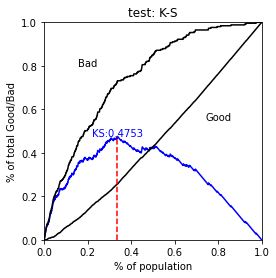
\includegraphics[scale=0.90]{figs/ks_plot.png}
%	\caption{KS Plot \label{ks_plot}}
%\end{figure}
%
%\begin{figure}[!ht]
%	\centering
%	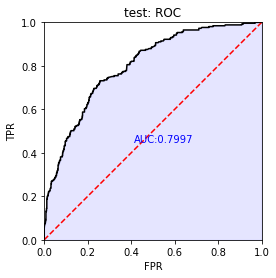
\includegraphics[scale=0.90]{figs/roc_plot.png}
%	\caption{ROC Plot \label{roc_plot}}
%\end{figure}

\begin{landscape}
\begin{figure}[!ht]
\begin{center}
	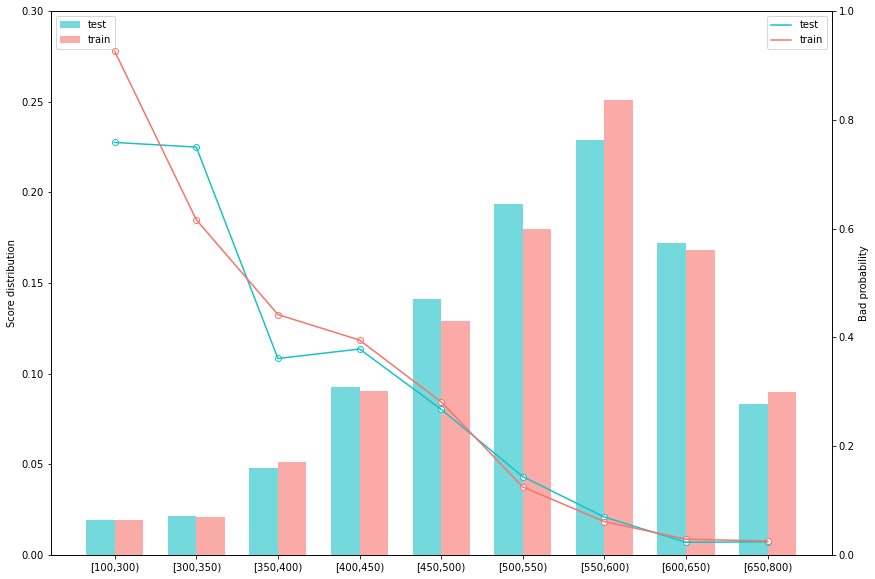
\includegraphics[scale=0.70]{figs/scorecard_plot.png}
	\caption{Scorecard Plot \label{scorecard_plot}}
\end{center}
\end{figure}
\end{landscape} 

\begin{figure}
\centering
  \centering
  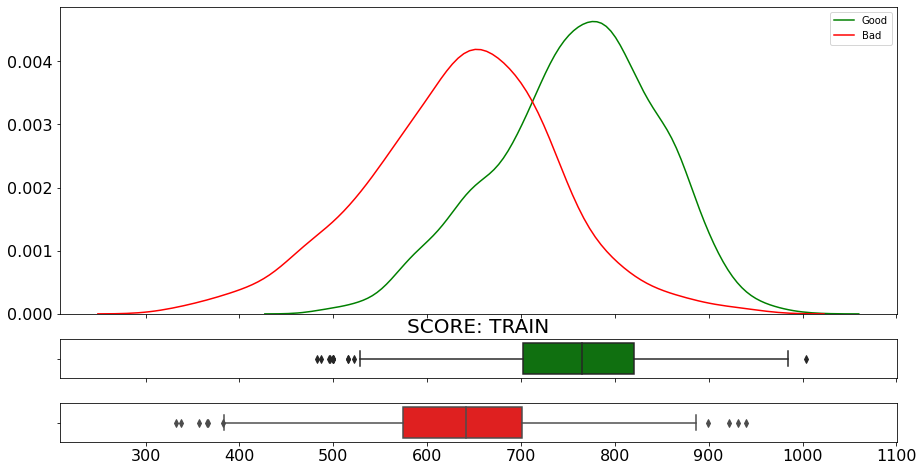
\includegraphics[width=0.9\linewidth]{figs/scorecard_dist_train.png}
  \caption{Scorecard Distribution for Train data}
  \label{fig:sc_dist_train}
\end{figure}

\begin{figure}
\centering
  \centering
  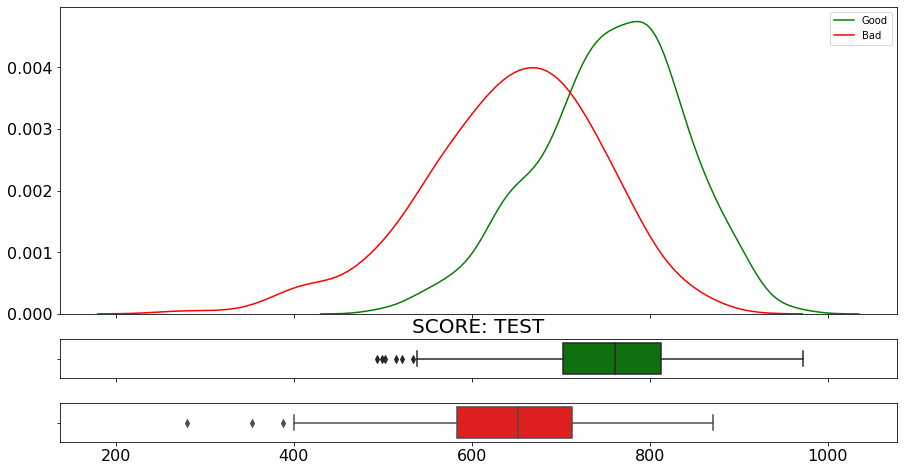
\includegraphics[width=0.9\linewidth]{figs/scorecard_dist_test.png}
  \caption{Scorecard Distribution for Test data}
  \label{fig:sc_dist_test}
\end{figure}
